\begin{savequote}[75mm]
   You know nothing, Jon Snow.
\qauthor{Ygritte, A Song of Ice and Fire by George R. R. Martin}
\end{savequote}

\chapter{Wprowadzenie}
\newthought{Skąd wzięły się planety?} Pytanie które nurtuję ludzkość od
zamierzchłych czasów. Konkretne rozważania teoretyczne dotyczące pochodzenia
planet mają długą historię sięgającą przynajmniej XVIII wieku, kiedy to Immanuel
Kant wysunął \dq{}Hipotezę mgławicową\dq{}. Już wtedy unikalność Układu
Słonecznego stanowiła przedmiot debaty. Dopiero na początku XX wieku pogląd, iż
układy planetarne są czymś powszechnym we Wszechświecie, został zaakceptowany
przez środowisko naukowe, a w roku 1992 została odkryta pierwsza, pozasłoneczna
planeta orbitująca pulsar PSR 1257+12 b~\cite{1992Natur.355..145W}.

W połowie XVIII wieku, filozof francuski Immanuel Kant zasugerował, iż rozmyte
o\-biek\-ty obserwowane przez niego przez teleskop mogą być wyspowymi
Wszechświatami takimi jak nasz, bądź obłokami materii w których formują się
gwiazdy i planety~\cite{ImmanuelKant.etal:2008}. $\ldots$ $\ldots$

%\begin{figure}[!ht]
%\centering
%\includegraphics[width=0.8\textwidth]{figures/laplace.png}
%\caption{Model mgławicy Laplace'a: (a) rotująca mgławica; (b) kolapsująca
%mgławica ulega spłaszczeniu wzdłuż osi rotacji; (c) soczewkowaty kształt
%mgławicy; (d) pierścienie materii pozostawione przez zapadający się obiekt
%centralny; (e) zagęszczenia na poszczególnych pierścieniach kolapsują tworząc
%planety. (Obrazek z pracy Woolfson, 1993)} 
%\label{fig:laplace}
%\end{figure}

\section{Paradygmat formowania się planet}
\subsection{Narodziny gwiazdy}
Formowanie się planet jest nierozerwalnie związane z narodzinami gwiazd, które
biorą swój początek w gęstych pyłowo--gazowych obłokach materii. Zanurzone w
gorącym ośrodku międzygwiazdowym, początkowo w stanie równowagi termodynamicznej
z otaczającym je gazem, obłoki takie często występują w ogromnych kompleksach i
obserwowane są jako ciemne mgławice molekularne~\cite{Tielens05}. W ich pobliżu
odnajdywane są gwiazdy~\emph{T Tauri} -- obiekty zmienne o jasności większej niż
wynikałoby to z ich temperatur efektywnych, co sugeruje ich młody wiek, nie
przekraczający 1~\Myr~\cite{H62}. Obserwowane temperatury efektywne sugerują, iż
we wnętrzach nie panują dostatecznie wysokie temperatury aby, mogły zachodzić
już reakcje spalania wodoru~\cite{CK79}. Część z obserwowanych gwiazd T~Tauri
jest częściowo zanurzona w małych, ciemnych i gęstych obłokach materii. Jak
pokazują obserwacje na falach radiowych i w podczerwieni, obłoki te są na tyle
gęste że siła wynikająca z ich samograwitacji jest w stanie zrównoważyć siłę
pochodzącą od gradientu ciśnienia~\cite{WT02}. Ich wewnętrzna struktura jest
wysoce hierarchiczna, tzn. we wnętrzu pojedynczego gęstęgo obłoku o masach rzędu
tysięcy mas słonecznych rozciągającego się na wiele parseków, znajdują się dużo
gęstsze obiekty o masach rzędu $1\Msun$ i rozmiarach rzędu $0.1\pc$~\cite{M85,
LSM93}. Obserwacje rotacyjnych linii emisyjnych molekuły NH$_3$ pozwalają
szacować typowe koncentracje gazu w obłokach na $10^{4}\cm^{-3}$~\cite{BM89}.
Nieregularny brzeg obłoków w połączeniu z ich, w przybliżeniu,
fraktalną strukturą interpretowany jest jako obecność silnej turbulencji w
samych obłokach~\cite{E00, FPW91}. Nie jest jasne czy ta struktura jest
przejściowym etapem ewolucji całego kompleksu obłoków, czy też
quasi-stacjonarnym stanem~\cite{L94}. Obecnie uważa się, że głównym źródłem
turbulencji jest pole magnetyczne, zaś obserwowane struktury są następstwem
rozchodzących się fal Alvena~\cite{NP03, MLK04}.
Typowe temperatury obłoków molekularnych wynoszą od 10 do 20\K. Za efektywne
chłodzenie początkowo odpowiada emisja w podczerwieni molekuły CO~\cite{MSWG82},
jednakże w trakcie kolapsu grawitacyjnego gaz sprzęga się termicznie z pyłem,
który wypromieniowuje nadwyżkę energii w podczerwieni~\cite{HN65, MI00} przez co
temperatura całego zapadającego się obłoku pozostaje stała.

\par Procesy zachodządze w samych obłokach tj. turbulencja, samograwitacja, lub
w ośrodku zewnętrznym tj.  wybuchy supernowych mogą powodować wzrost gęstości
poszczególnych zagęszczeń w obłoku. W momencie w którym obszar gęstej materii
przekroczy  masę krytyczną, nazywaną masą Jeansa $M_J$~\cite{J1902, J1928},
grawitacja przeważa i chmura zaczyna się zapadać (rysunek 1a). Masa Jeansa
zależy od temperatury kinetycznej ośrodka $T$ oraz jego gęstości
$\rho$~\cite{H64} 

\begin{equation} M_J \sim
   \left( \frac{k_B T}{G} \right) ^\frac{3}{2} {\rho}^{-\frac{1}{2}},
\end{equation} 
gdzie $k_B$ jest stałą Boltzmanna a $G$ jest stałą grawitacji.
Dla typowych warunków panujących wewnątrz obłoków materii
międzygwiazdowej~\cite{BM89}, masa Jeansa przyjmuje wartość

\begin{equation}
 M_J \approx 2.9 M_{\odot} \left(\frac{T}{10\K}\right)^{1.5} 
 \left(\frac{n}{10^4\cm^{-3}}\right)^{-0.5},
\end{equation}
gdzie $n = \rho_g / \mu \mH$ jest koncentracją cząstek materii.
W wypadku braku ciśnienia, kolaps obłoku następowałby w tzw. skali czasowej
spadku swobodnego~\cite{Spitzer1978}
\begin{equation}
   t_{\textrm{ff}} \sim \frac{1}{\sqrt{G\rho}} \sim 10^5\yr
   \left(\frac{n}{10^4\thinspace \cm^{-3}}\right)^{-0.5}.
\end{equation}
W rzeczywistości gradient ciśnienia w niewielkim tylko stopniu spowalnia
zapadanie się materii~\cite{T82}. Obliczenia numeryczne pokazują, że gęstość
materii w zapadającym się obłoku asymptotycznie zbiega do $\rho \propto
r^{-2}$~\cite{L69}. W rezultacie tylko niewielka część masy obłoku formuje
protogwiazdę, reszta materii zostaje uwięziona w formie rozciągniętej otoczki
opadającej na obiekt centralny. Przy braku rotacji i zaniedbaniu wpływu pola
magnetycznego otoczka opada radialnie w tempie~$\propto c_s^3 / G$, gdzie
$c_s$ jest izotermiczną prędkością dźwięku. Stała proporcjonalności wynosi od
kilkadziesiąt~\cite{H77} do około jedności~\cite{S77}.
\par Jak już wcześniej wspomniano, pole magnetyczne odgrywa istotną rolę w
dynamicznej ewolucji całego kompleksu obłoków molekularnych i należy spodziewać
się silnej obecności pola magnetycznego w zapadającym się obłoku molekularnym i
jego przeciwdziałania wobec siły samograwitacji~\cite{MC99}. Początkowa
kondensacja materii w centrum grawitacji jest możliwa dzięki dyfuzji
ambipolarnej, która zachodzi w skalach czasowych rzędu $10^7$~lat~\cite{MZGH93}.
Dzięki stopniowemu zwiększaniu masy, centralna część podtrzymywanego przez pole
magnetyczne obłoku ulega powolnej kontrakcji do momentu osiągnięcia koncentracji
materii rzędu $10^{-3}\cm^{-3}$, dla której siła samograwitacji przeważa nad
ciśnieniem magnetycznym i rozpoczyna się nieograniczony kolaps~\cite{BM94, CB00}.
Ostatnie eksperymenty numeryczne~\cite{JHCF13} sugerują, że uwzględnienie
wpływu turbulencji pod czas kolapsu pozwala efektywniej przełamać
przeciwdziałający samograwitacji wpływ pola magnetycznego, nawet dla silnie
namagnesowanego ośrodka.
\par We wcześniejszych rozważaniach całkowicie zaniedbano wpływ rotacji na
ewolucję formującej się protogwiazdy. Większość obserwowanych obłoków materii z
której formują się potem gwiazdy rotuje~\cite{GBFM93}, co wydaje się być
naturalną konsekwencją turbulencji obecnej w obłokach~\cite{BB00}. Typowy
moment pędu obserwowany w obłokach protogwiazdowych jest przynajmniej o rząd
większy, niż ten który mogła by wytrzymać gwiazda rotując z maksymalną
prędkością równoważącą siłę samograwitacji. Fakt ten implikuje istnienie
mechanizmu odpowiedzialnego za transport momentu pędu, o którym będzie mowa w
dalszej części tej pracy. Uwzględnienie rotacji w modelowaniu protogwiazd,
prowadzi do wniosku, że materia nie opada centralnie na centrum grawitacji, lecz
formuje dysk podtrzymywany przez równowagę pomiędzy radialną składową siły
grawitacji oraz siłę odśrodkową~\cite{TSC84}. Biorąc pod uwagę
masę opadająca z otoczki, formujący się dysk jest na granicy stabilności, bądź
jest całkowicie niestabilny grawitacyjnie~\cite{SKBT94}. W rezultacie tworzą
się w nim spiralne fale grawitacyjne, które na skutek \emph{gravitational
torques} napędzają akrecję materii na protogwiazdę~\cite{St00}. W tym
scenariuszu fluktuacje gęstości muszą jednak saturować się na odpowiednio niskim
poziomie aby dysk nie rozpadł się, nie jest do końca jasne czy w takich
warunkach możliwe jest osiągnięcie quasi-stacjonarnego stanu równowagi. W
przeciwnym wypadku dysk ulega fragmentacji tworząc układ podwójny lub
wielokrotny. Ewolucja masywnego dysku zostanie dokładnie opisana w
podrozdziale~\ref{sec:GI}. 

\par Formujące się w centrum zagęszczenie staje się nieprzezroczyste dla
termicznej emisji pyłu dla gęstości gazu większej niż $10^{-13}\g\cm^{-3}$
$(2\cdot10^{10}$ H$_2\cm^{-3})$~\cite{L69} i temperatura wnętrza obłoku zaczyna
rosnąć. Kończy to etap izotermicznego kolapsu. Nieprzezroczyste jądro obłoku
staje się adiabatyczne (wykładnik adiabatyczny H$_2$: $\gamma = 7/5$~\cite{L69})
dla gęstości powyżej $10^{-12}\g\cm^{-3}$. Ciśnienie skompresowanego gazu staje
się coraz bardziej istotne i prowadzi do praktycznie całkowitego zatrzymania
kolapsu dla gęstości centralnej $\sim 2\cdot 10^{-10}\g\cm^{-3}$ osiągając
równowagę hydrostatyczną. Masa z otoczki nie przestaje być jednak akreaowana i
gęstość oraz temperatura jądra cały czas rośnie. Krytycznym momentem jest
osiągnięcie przez gaz temperatury $2000\K$, dla której następuje dysocjacja
molekuły H$_2$ i gwałtowny spadek wykładnika adiabatycznego poniżej wartości
$4/3$. Ta druga faza kolapsu zachodzi w podobny sposób jak początkowy
kolaps izotermiczny. Trwa aż do momentu kiedy wodór zostanie zjonizowany przez
wzrost temperatury i wykładnik adiabatyczny gazu wzrósnie do wartości $5/3$.
Wzrost ciśnienia pozwala na uformowanie drugiego jądra pozostającego w
równowadze hydrostatycznej. Posiada ono dość nie wielką masę rzędu
$10^{-3}\Msun$ i rozmiar około $1\Rsun$~\cite{MI00}. Całkowita masa formującej
się protogwiazdy nie przekracza na tym etapie $10^{-2}\Msun$. Dominującym
procesem staje się akrecja materii, która musi dostarczyć pozostałe 99\% masy do
rodzącej się gwiazdy. 

W trakcie akrecji, protogwiazda cały czas pozostaje niewidoczna dla obserwatora,
przysłonięta przez pył znajdujący się w opadającej otoczce. Klasyfikacja
obserwacyjna takiego układu kreśla obiekty na tym etapie mianem \emph{klasy
0}~\cite{andre} (rysunek 1b). Ich obserwowana temperatura jest stosunkowo niska
$(T \lesssim 30\K)$. Obiekty tej klasy charakteryzują się maksimum w rozkładzie
energii promieniowania wypadającym w dalekiej podczerwieni, bez wykrywalnej
nadwyżki w bliskiej podczerwieni. Z czasem kiedy z otoczki ubywa materii,
obszar optycznie gruby staje się coraz mniejszy i maksimum wypromieniowywanej
energii przesuwa się w kierunku bliższej podczerwieni. Ostatecznie
światło samej gwiazdy przebija sie przez pozostałość otoczki dzięki czemu można
zaobserwować charakterystyczne, dwuskładnikowe widmo (patrz
Rysunek~\ref{fig:sed}). Obserwatorzy wprowadzili prostą klasyfikację tak młodych
obiektów dzieląc je na 4 klasy: 0, I, II i III, które oznaczają położenie
maksimum w rozkładzie energii promieniowania odpowiednio na falach:
submilimetrowych, dalekiej podczerwieni, bliskiej podczerwienie i w zakresie
widzialnym. Poszczególne klasy odpowiadają też różnym fazom akrecji materiału i
różnią się długością trwania. Protogwiazdy znajdują się w klasie 0 przez około
kilkadziesiąt tysięcy lat~\cite{FSSK06}. W tym czasie następuje gwałtowna
akrecja materii.  Klasa I jest o rząd dłuższa (kilka $10^5$ lat), zaś maksymalny
wiek obserwowanych gwiazd T Tauri (klasa II) wynosi $10^6$ lat~\cite{HCGD98}.
Dla obiektów klasy III w obserwowanych widmach zanikają wszelkie struktury
przypisywane materii wokołogwiazdowej~\footnote{ang. \emph{weak-line T Tauri
stars}}. Protogwiazda traci materię z dysku na skutek jego
fotoewaporacji~\cite{ACP06} i wiatru gwiazdowego~\cite{PN86}. Wiele
obserwowanych gwiazd T Tauri wykazuje w obserwowanych widmach już tylko
szczątkową akrecję $10^{-7} \div 10^{-8} \Msun\yr^{-1}$~\cite{Hart98}. Tak niski
poziom akrecji nie jest już w stanie znacząco wpłynąć na masę gwiazdy i proces
jej formowania można uznać za zakończony.

\subsection{Core Accretion}

Z punktu widzenia teorii formowania się planet, w układzie rodzącej się
protogwiazda i materii która ją otacza, kluczowa jest ewolucja
wokółgwiazdowego dysku akrecyjnego. Jego dyspersja wyznacza ostateczna granicę
czasową, do której procesy formacji planet muszą się zakończyć. Hipotezę 

Ewolucję pyłu można podzielić na zgrubsza na 4 etapy:

\begin{figure}[p]
\centering 
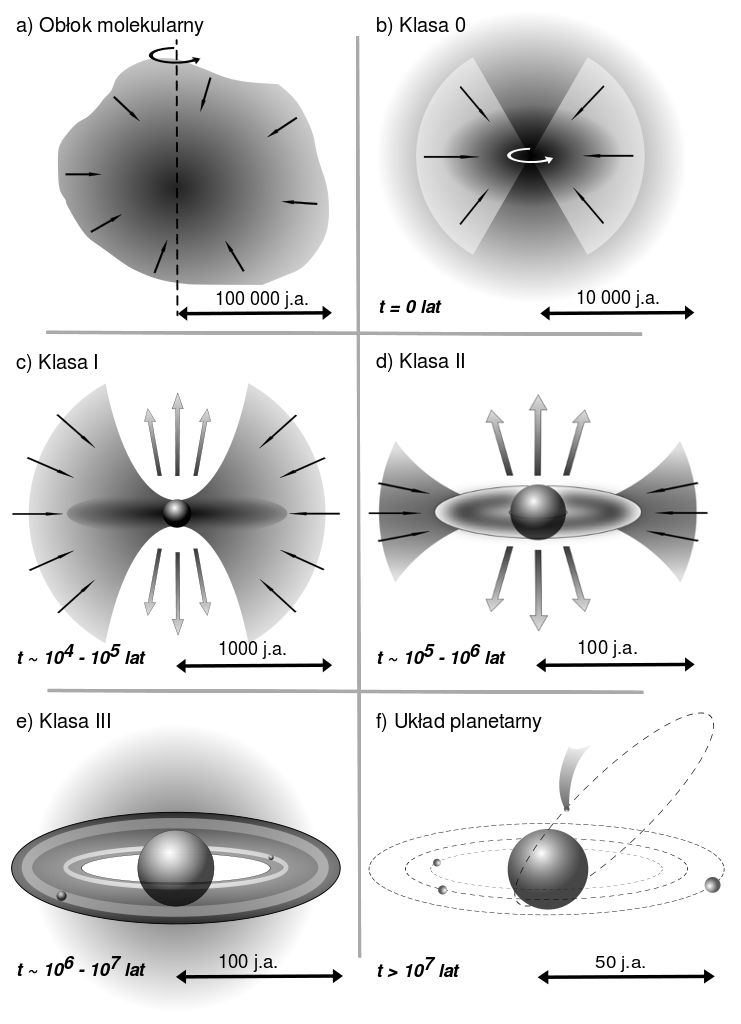
\includegraphics[width=0.9\textwidth]{figures/planetformation.png}
\caption{Ilustracja przedstawia kolejne fazy formowania się mało masywnej gwiazdy
   wraz z systemem planetarnym: a) kolaps grawitacyjny gęstego obłoku; b)
   oddziaływanie centralnego pola grawitacyjnego oraz siły odśrodkowej powoduje
   opadanie materii i formowanie się dysku; c) faza FU Orionis: silna akrecja w
   dysku oraz wypływ materii w okolicach osi obrotu; d) faza T Tauri: zmniejsza
   się tempo akrecji $\sim 10^{-8}\Msun\yt^{-1}$ oraz wypływu materii,
   rozpoczyna się proces formowania planet; e) zanika składowa gazowa, planety
otwierają przerwy w dysku, następuje również ich migracja; f) cały gaz oraz
mniejsze ciała zostają pochłonięte przez planety lub usunięte z dysku, układ
planetarny przyjmuje ostateczny kształt.}

\label{fig:planet}
\end{figure}

\begin{description}
   \item[i) koagulacja ziaren pyłu $\left(\mum \rightarrow \km\right):$] 
      Z doświadczeń laboratoryjnych wynika~\cite{BW08}, że drob\-ne cząsteczki pyłu
      mogą na skutek wzajemnych zderzeń zwiększać swoje rozmiary. ,,Spoiwem'' stają
      się siły van der Waalsa bądź oddziaływanie elektrostatyczne. Opierając się
      na analizie drogi swobodnej jednorodnej frakcji cząstek pyłu o promieniu
      $a$, można określić charakterystyczną skalę czasową koagulacji jako 

   \begin{equation}\label{coag} 
      t_{\textrm{coag}} % = \frac{1}{n_d \sigma \Delta v}
      \sim \frac{a}{\Delta v}\frac{\rho_p}{\rho_d} \approx 
      10^{-12} \rho_d^{-1}\yr\thinspace
      \left(\frac{a}{1\mum}\right)
      \left(\frac{\Delta v}{0.1\m\s^{-1}}\right)^{-1}
      \left(\frac{\rho_p}{3\g\cm^{-3}}\right),
   \end{equation}

   gdzie $\Delta v$ jest średnią prędkością względna cząstek, $\rho_p$ jest
   gęstością materiału budującego cząstki natomiast $\rho_d$ jest gęstością
   ośrodka pyłowego w dysku.  Biorąc pod uwagę typowe gęstości pyłu w obłokach
   gwiazdowych $(\rho_d \sim 10^{-20}\g\cm^{-3})$ proces ten
   zachodzi w skali czasowej milionów lat. Jednakże dla dysków protoplanetarnych
   o typowych gęstościach rzędu $10^{-10}\g\cm^{-3}$\footnote{jest to całkowita
   gęstość z uwzględnieniem obu składników: gazu i pyłu. Przyjmuje się że
kanoniczna wartość stosunku gęstości pyłu do gęstości gazu $\epsilon$ wynosi
0.01. Zatem $\rho_d \sim 10^{-12}\g\cm^{-3}$} proces
koagulacji zachodzi w skalach lat czy tez dziesiątek lat i może bardzo szybko
prowadzić do wytworzenia się planetezymali. W rzeczywistości dla ziaren pyłu o
rozmiarach decymetrów czy metrów pojawia się szereg procesów przeciwdziałających
dalszemu wzrostowi, a także ulega zmianie średnia prędkość względna cząstek pyłu
zmieniając prawdopodobieństwo wyniku kolizji na korzyść fragmentacji raczej niż
koagulacji.  

\item[ii) oligarchiczny wzrost $\left(\km \rightarrow
   10^3\km\right)$:]
   Faza druga formowania się planet rozpoczyna się w momencie w którym przeważa
   wzajemne oddziaływanie grawitacyjne pomiędzy planetezymalami i to grawitacja
   staje się nowym spoiwem łączącym zderzające się obiekty. Tarcie
   aerodynamiczne jest nadal niezaniedbywalne i zapewnia kołowość orbit
   planetezymali, co zwiększa szanse na zderzenia.
\item[iii) akrecja gazu]
   Po osiągnięciu rozmiarów rzędu $10^3\km$ jądra planetarne
   są w stanie wiązać grawitacyjnie gaz na swoich powierzchniach. Globalne
   oddziaływanie dysk $\iff$ planety staje się istotne i może prowadzić z jednej
   strony do migracji planet, a z drugiej strony do otworzenia się przerw w
   dysku~\citep{KKI06}.
\item[iv) długoskalowa ewolucja dynamiczna:]
   Faza zdominowana tylko i wyłącznie przez wzajemne oddziaływanie grawitacyjne
   pomiędzy utworzonymi planetami, a także z gwiazdą macierzystą. Układ
   planetarny może na tym etapie utracić znaczną część masy pyłowej, poprzez
   pochłonięcie planety przez gwiazdę, bądź wprowadzenie jej na orbitę
   hiperboliczną.
\end{description}
Powyższy scenariusz formowania się planet nosi nazwę modelu ,,akrecji na
jądra''~\footnote{ang. \emph{core-accretion}}. Alternatywną teorią, szczególnie
wdzięcznie wyjaśniająca powstawanie gazowych olbrzymów w masywnych dyskach
protoplanetarnych, jest model zakładający kolaps i fragmentację grawitacyjną
dysku~\cite{Boss97}. Zostanie ona omówiona w dalszej części tego rozdziału.

\section{Ważne pojęcia}
Gazowo--pyłowy dysk, który powstaje podczas kolapsu obłoku protogwiazdowego jest
miejscem w którym powstają planety. Pewne szczególne mechanizmy oraz globalna
dynamika mogą temu procesowi pomagać, bądź mu przeciwdziałać. Poniższe akapity
pokrótce opisują strukturę dysku protoplanetarnego oraz najważniejsze efekty
dynamiczne związane z samym gazem, następnie przechodząc do ich wpływu na
dynamikę i ewolucję pyłu. Pozwoli to wskazać problemy z jakimi boryka się model
,,akrecji na jądra'' i naturalnie przejść do celu tej rozprawy.

\subsection{Struktura dysku protoplanetarnego}
Proces kolapsu grawitacyjnego, sferycznego obłoku materii międzygwiazdowej nie
wpływa na jego całkowity moment pędu. Przy założeniu, że obłok rotuje, nawet
bardzo wolno, to materia nie opada bezpośrednio na obiekt
centralny, lecz formuje dysk w płaszczyźnie prostopadłej do wektora całkowitego
momentu pędu. Aby określić przybliżone warunki fizyczne w formującym się dysku
możemy posłużyć się równaniami hydrodynamiki:

\begin{gather}
   \partial_t \rho_g + \nabla\cdot\left(\rho_g\mathbf{u}\right) = 0,
   \label{eq:hd1}\\
\partial_t \mathbf{u} + \left(\mathbf{u}\cdot\nabla\right)\mathbf{u} = 
-\nabla\Phi + -\frac{1}{\rho_g} \nabla P \label{eq:hd2}
\end{gather}

gdzie $\rho_g$ jest gęstością gazu, $P$ ciśnieniem, 
związanych z tarciem, a $\Phi$ potencjałem grawitacyjnym. Jeżeli ponadto
założymy, że dysk:

\begin{enumerate}
   \item jest izotermiczny to $P = c_s^2 \rho_g \implies -\frac{1}{\rho_g}\nabla
      P = -c_s^2\nabla\ln\rho_g$, gdzie $c_s = \sqrt{\frac{k_{\textrm{B}} T}{\mu
    \mH}}$ jest izotermiczną prędkością dźwięku.
   \item jest stacjonarny i znajduję się w równowadze hydrostatycznej w kierunku
      $z$ to wertykalne przyspieszenie grawitacyjne $\partial_z \Phi = g_z =
      (GM_\star/r^2) z/r = \Omega^2 z$, gdzie $M_\star$ to masa gwiazdy
      macierzystej, $\Omega$ orbitalna częstość keplerowska, $G$ stała
      grawitacji Newtona, jest równoważone przez siłę wynikająca z gradientu
      ciśnienia gazu $\partial_z P / \rho_g$
\end{enumerate}

Łącząc powyższe założenia otrzymujemy rozkład gęstości gazu

\begin{equation} \label{eq:zeq}
   \rho_g(z) = \frac{\Sigma_G}{H\sqrt{2\pi}} \exp \left[
   \frac{1}{2}\left(\frac{z}{H}\right)^2 \right],
\end{equation}

gdzie $\Sigma_g = \int \rho_g(z) dz$ jest gęstością powierzchniową, a
$H=\frac{c_s}{\Omega}$ to charakterystyczna skala grubości dysku.

%\par Zakładając w pierwszym przybliżeniu że dysk jest optycznie gruby, t.j.
%absorbuję całkowicie promieniowanie pochodzące od gwiazdy i następnie reemituje
%je jako ciało doskonale czarne, można pokazać~\cite{armitage07} że $T \propto
%r^{-3/4}$ i co za tym idzie $c_s \propto r^{-3/8}$. Dokładniejsze szacunki,
%które lepiej oddają obserwowane dystrucje spektralne energii, można znaleźć w
%pracach~\cite{KenyonHART87, ChaingGold97} {\bf patrz armitage}.
%{\bf Tu raczej trzeba przedstawić tę wersję z której wynika $T \propto
%r^{-1/2}$}
%
\par W modelu stacjonarnym w kierunku radialnym grawitacja i siła wynikająca z
gradientu ciśnienia jest równoważona poprzez siłę odśrodkową
\begin{equation}\label{eq:radial_balance}
\frac{u_\phi^2}{r} = \frac{GM_\star}{r^2} +
  \frac{1}{\rho_g}\frac{\textrm{d}P}{\textrm{dr}},
\end{equation}
gdzie $u_\phi$ jest prędkością orbitalną gazu. Wpływ gradientu ciśnienia na
globalną dynamikę jest znikomy (rzędu $O(H/r)^2$), dlatego dla cienkich dysków
$(H/r \ll 1)$ z dobrym przybliżeniem można przyjąć, że właściwy moment pędu dla
gazu jest równy momentowi pędu wynikającemu z ruchu keplerowskiego. Z równania
\mref{eq:radial_balance} wynika zatem, że moment pędu jest rosnącą funkcją
promienia:
\begin{equation}\label{eq:angmom}
l = r^2\Omega = \sqrt{GM_\star r}.
\end{equation}
Z równania \mref{eq:angmom} wypływa niezwykle ważny fakt: aby materiał z dysku
mógł być akreaowany przez gwiazdę macierzystą, w układzie musi działać mechanizm
powodujący utratę bądź chociaż redystrybucję momentu pędu.
\subsection{Niestabilność magnetorotacyjna}
Z obserwacji jasno wynika~\citep{MME04}, że dyski
protoplanetarne nie są obiektami stacjonarnymi. Co więcej, obiekty klasy I
posiadają wysokie tempa akrecji $\sim 10^{-5}\Msun\yr^{-1}$. Aby zapewnić
radialny przepływ materii w kierunku gwiazdy macierzystej, potrzeba wprowadzić
efektywny mechanizm transportu momentu pędu. W tym celu musimy odejść od
przybliżenia hydrodynamiki dla idealnego gazu i zastosować równania
Naviera-Stokesa, które rozszerzają równanie ruchu~\ref{eq:hd2} o tensor naprężeń
płynu

\begin{gather}
   \partial_t \rho_g + \nabla\cdot\left(\rho_g\mathbf{u}\right) = 0,
   \label{eq:ns1}\\
\partial_t \mathbf{u} + \left(\mathbf{u}\cdot\nabla\right)\mathbf{u} = 
-\nabla\Phi -\frac{1}{\rho_g} \nabla P + \frac{1}{\rho_g} \nabla \cdot \Pi.
\label{eq:ns2}
\end{gather}
Jeżeli dodatkowo założymy, że mamy do czynienia z płynem doskonale lepkim, tensor
naprężeń można zredukować do postaci $\Pi = (\rho_g \nu)\nabla\cdot\mathbf{u}$,
gdzie $\nu$ jest lepkością kinematyczną. Całkując układ
równań~\mref{eq:ns1}-\mref{eq:ns2} w kierunku wertykalnym i dokonując prostych
przekształceń można otrzymać
\begin{equation}\label{eq:sigma}
   \partial_t \Sigma_g =
   \frac{3}{R}\partial_R\left(\frac{1}{R\Omega}\partial_R\left(R^2\Sigma_g \nu
         \Omega\right)\right).
\end{equation}
Rozwiązaniem stacjonarnym równania~\mref{eq:sigma} jest warunek $\Sigma_g\nu =
\textrm{const}$, co przekłada się na tempo akrecji $\dot{M} = 3\pi\Sigma_g\nu$.
Z powyższego warunku wynika, że lepkość jest kluczowym elementem napędzającym
akrecję materii. Problemem pozostaje jakie proces fizyczny jest za nią
odpowiedzialny?
\par Podstawowa lepkość, tj. lepkość molekularna $\nu_{\textrm{m}} \sim c_s
\lambda$, gdzie $\lambda = 1 / n\sigma$ to średnia droga swobodna molekuł gazu,
zaś $n$ to koncentracja molekuł gazu, a $\sigma$ ich przekrój czynny, dla
typowych wartości gęstości i temperatury dysków protoplanetarnych wynosi
$\nu_{\textrm{m}}\sim10^5\cm^2\s^{-1}$~\cite{armitage}. Przekłada się to na
tempo akrecji na poziomie $\dot{M}\sim 10^{-17}\Msun\yr^{-1}$. Co więcej
charakterystyczna skala czasowa takiego procesu $\tau \simeq R^2 /
\nu_{\textrm{m}}$ wynosi $10^{13}\yr$. Z tego względu lepkość molekularną można
całkowicie zaniedbać w dalszych rozważaniach.
\par W słynnej pracy Shakura \& Sunyaev~\citep{SS73} zauważyli, że turbulencja
w dysku może być dobrym źródłem lepkości, znacznie wydajniejszym niż lepkość
molekularna. Dla izotropowej turbulencji, maksymalna skala wirów w dysku jest
proporcjonalna do charakterystycznej skali grubości dysku $H$, zaś maksymalna
prędkość ruchu turbulentnych jest rzędu prędkości dźwięku, ponieważ fale
uderzeniowe bardzo szybko dyssypują energię kinetyczną. Shakura \& Sunyaev
zaproponowali parametryzację lepkości turbulentnej

\begin{equation}\label{eq:alpha}
\nu = \alpha c_s H
\end{equation}

, gdzie $\alpha$ jest bezwymiarowym parametrem określającym wydajność
turbulencji w transporcie momentu pędu. Aby wyjaśnić obserwowane tempo akrecji
dla gwiazd \emph{T Tauri}, parametr $\alpha$ powinien być rzędu $10^{-2}$.
Problem dalej pozostaje źródło turbulencji w dysku. Z kryterium
Rayleigha

\begin{equation}
   \frac{\mathrm{d}}{\mathrm{d}r}\left(r^2\Omega\right) > 0,
\end{equation}

wynika że hydrodynamiczny dysk keplerowski jest liniowo stabilny. Sytuacja
diametralnie się zmienia w jeżeli uwzględnimy obecność w układzie dowolnie
słabego pola magnetycznego. Balbus \& Hawley~\citep{BH91} pokazali, że przepływ
magnetohydrodynamiczny jest stabilny liniowo wtedy i tylko wtedy, gdy

\begin{equation}\label{eq:mri}
   \frac{\mathrm{d}}{\mathrm{d}r}\left(\Omega^2\right) > 0.
\end{equation}
Warunek \mref{eq:mri} \emph{nie jest} spełniony dla dysków keplerowskich. W
rezultacie nawet szczątkowe pole magnetyczne, jest w stanie wzmocnić wykładniczo
zaburzenia gęstości w gazie w dynamicznej skali czasowej, powodując silną
turbulencję. Proces ten określany jest mianem niestabilności magnetorotacyjnej
(MRI). Co więcej, zarówno symulacje lokalne~\cite{DSP10} jak
i globalne~\cite{FD11} szacują współczynnik $\alpha$ wynikający z turbulencji
wzbudzonej przez MRI na $\alpha\sim 10^{-2}$.
\par Należy zauważyć, że niestabilność magnetorotacyjna wymaga choć szczątkowego
zjonizowania gazu. Jeżeli założymy że źródłem jonizacji jest wysoko energetyczne
promieniowanie pochodzące od gwiazdy macierzystej i weźmiemy pod uwagę strukturę
pionową dysku~\mref{eq:zeq}, to dojdziemy do wniosku iż od pewnej wysokości
$H_i$ dysku gaz znajdujący się poniżej $(H < H_i)$ jest efektywnie osłaniany
przez warstwy gazu o $H > H_i$. Obszar $H < H_i$ jest zatem \emph{martwą strefą}
w której turbulencja wzbudzana przez MRI nie występuje~\cite{DFT10}.

\begin{figure}
   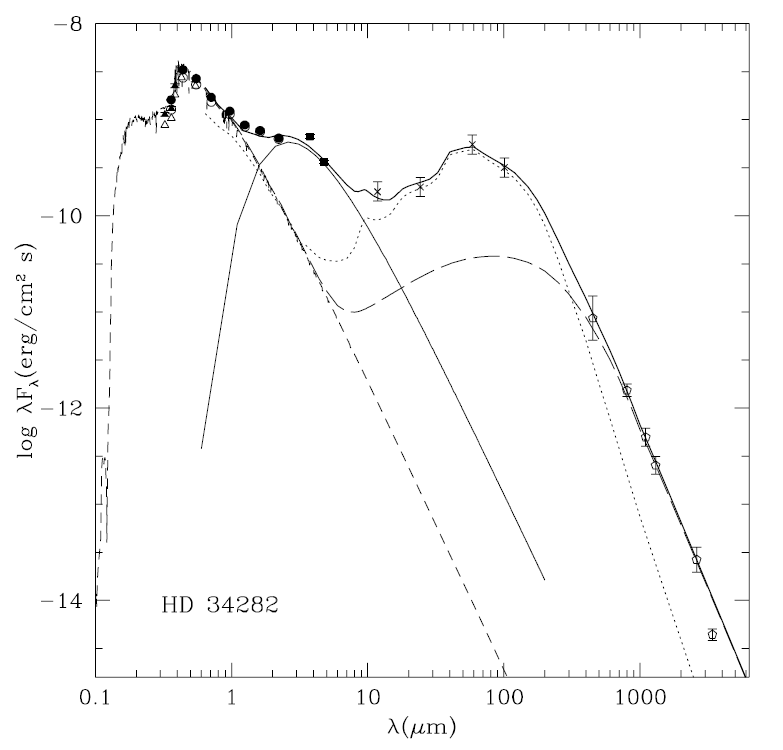
\includegraphics[width=0.9\textwidth]{figures/chap1_sed.png}
   \caption{Rozkład widma energii dla gwiazdy HD 34282. Symbole oznaczają
      obserwacje różnymi metodami dla odpowiednich długości fali. Do obserwacji
      dopasowano następujące modele: linia przerywana model widma gwiazdowego
      dla obiektu typu A3V $(T\sim 8600\K)$, cienka ciągła
      linia model ciała doskonale czarnego dla $T=1400\K$,
      linia kropkowana reprezentuje model dysku o nachyleniu $i=56^o$, tempie
      akrecji $\dot{M} = 8.2\times10^{-9}\thinspace\Msun\yr^{-1}$
      rozciągającym się od $0.31\AU$ do $705\AU$.
   Obrazek pochodzi z pracy~\cite{MME04}}
   \label{fig:sed}
\end{figure}

\subsection{Niestabilność grawitacyjna}
\label{sec:GI}
Dla odpowiednio masywnych i zimnych dysków protoplanetarnych, samograwitacja
materii jest w stanie przeważyć nad stabilizującymi efektami ciśnienia gazu oraz
rotacji i spowodować kolaps, a następnie fragmentację dysku. Podatność układu na
niestabilność grawitacyjną przyjęło się określać poprzez parametr Toomre'a $Q$
wyrażony poprzez
\begin{equation}
   Q = \frac{c_s\Omega}{\pi G \Sigma} \sim 10^2 
   \left(\frac{T}{100\K}\right)^{0.5}
   \left(\frac{\Sigma}{10^3\g\cm^{-3}}\right)^{-1}
   \left(\frac{R}{1\AU}\right)^{-1.5}.
\end{equation}
Jeżeli $Q\lesssim1$ dysk może się rozpaść na szereg grawitacyjnie związanych
obłoków, które okrążając gwiazdę macierzystą będą akreaować coraz więcej
materii. Każdy z tych obłoków może na skutek dalszej kontrakcji przekształcić
się planety, w szczególności w gazowe olbrzymy takie jak Jowisz czy
Saturn~\cite{B00}. Mechanizm ten jest alternatywnym do akrecji na jądra,
procesem prowadzącym do uformowania się planet. Jednakże dla typowych wartości
$T$ i $\Sigma_g$ parametr $Q\gg 1$ dla wewnętrznych obszarów dysku. Zewnętrze
obszary powinny być bardziej podatne na niestabilność grawitacyjną, choć dalej
wymagają efektywnych procesów chłodzenia w dysku. 
{\bf opisać mechanizm we włóknach jeżeli to potrzebne}

\subsection{Oddziaływanie pomiędzy gazem, a pyłem}
Oddziaływanie pomiędzy pyłem a gazem odbywa się poprzez tarcie aerodynamiczne.
Charakterystyczną skalę czasową tego procesu można wyrazić jako

\begin{equation}
   \tau_f = \frac{mv_\textrm{pg}}{F_\textrm{D}},
\end{equation}

gdzie $m$ i $v_{\textrm{pg}}\equiv|\mathbf{u} - \mathbf{v}|$ to odpowiednio masa
i prędkość cząstek pyłu względem gazu, zaś $F_\textrm{D}$ to siła tarcia.
$\tau_f$ można interpretować jako czas potrzebny do wytracenia pędu cząstki pyłu
i zrównania jej prędkości z gazem. Siła $F_\textrm{D}$ jest definiowana w różny
sposób w zależności od rozmiaru ziaren pyłu. Dla cząstek pyłu o promieniu $a < 9
\lambda / 4$ siła tarcia wyraża się prawem Epsteina 
\begin{equation}
   F_\textrm{D} = \frac{4}{3}\pi a^2 \rho_\bullet \rho_G c_s v_\textrm{pg}, 
\end{equation}
gdzie $\rho_\bullet = 1.6\g\cm^{-3}$ jest gęstością materiału z którego
zbudowany jest pył. Dla ziaren pyłu porównywalnych z drogą swobodną molekuł
gazu siła tarcia wyraża się poprzez prawo Stokesa i jest zależna od liczby
Reynoldsa, co znacznie komplikuje jej postać. W ramach pracy skupiono się na
obszarach dysków rozciągających się relatywnie dużych promieni tj. $>2\AU$.
Biorąc pod uwagę, iż średnią drogę swobodną możemy wyrazić przez $\lambda_g =
4.2\times 10^4\textrm{ cm} (10^{-14}\textrm{ g cm}^{-3}/\rho_g) \approx (R/1
\textrm{AU})^{2.75}\cm$~\citep{W77,BT09}, gdzie$R$ jest odległością radialną od
centrum dysku, reżim Epstein ma zastosowanie dla dominującej części domeny
obliczeniowej nawet dla największych symulowanych przez nas ziaren pyłu. Skala
czasowa tarcia przyjmuję zatem następującą postać:
%
\begin{equation} 
   \tau_f = \frac{\rho_\bullet a} {\rho_g \sqrt{c_s^2 +
      |\mathbf{u} - \mathbf{w}|^2 }} \label{eq:tauf} 
\end{equation}
%
Źródłem różnicy względnej prędkości pomiędzy pyłem a gazem może być wiele
procesów, przede wszystkim turbulencja obecna w gazie, ale także radialny dryf
pyłu o którym będzie mowa w dalszej części tego rozdziału, oraz ruchy
brownowskie. Te ostatnie bardzo silnie zależą od rozmiaru cząstek, tj.
makroskopowe cząstki pyłu praktycznie nie odczuwają ich wpływu, nie są zaś
zależne od gęstości gazu. Ruch brownowskie są nie zwykle istotne dla rozpoczęcia
procesów koagulacji pyłu w początkowej fazie formacji
protoplanet~\citep{DD05}, jako że wzbudzają dość znaczne prędkości względne
dla najmniejszych ziaren pyłu, które są najsilniej związane z gazem. Turbulencja
i radialny dryf natomiast tym silniej pływają na dynamikę, im większa jest
gęstość gazu. Ich rola jest większa dla cząstek o rozmiarach pośrednich, które
zaczynają odprzęgać się od dynamiki gazu.

\subsection{Radialny dryf pyłu}
Pył w dysku protoplanetarnym można traktować jako bezciśnieniowy płyn. Ten
prosty fakt niesie za sobą ogromne konsekwencje. Jako że rozkład materii w dysku
jest malejącą funkcją promienia, to dla izotermicznego gazu gradient ciśnienia
jest ujemny dla całej rozciągłości dysku. W rezultacie gaz w jest efektywnie
ekranowany od siły grawitacyjnej. Z równowagi sił wynika
\begin{equation}
   R\Omega_g^2 = \partial_R P / \rho_G + R\Omega_K^2,
\end{equation}
że prędkość orbitalna dla gazu jest nieznacznie mniejsza niż prędkość
keplerowska. Niedobór prędkości rotacji gazu względem przyjęło określać się jako
$\eta v_\textrm{K}$, gdzie $\eta$ to bezwymiarowy parametr~\cite{N86}
wyrażony jako
\begin{equation}
   \label{eq:eta}
   \eta = \frac{\partial_R P}{2\rho_\textrm{G} R \Omega^2} = \frac{1}{2}
   \frac{c_s^2}{v_\textrm{K}^2} \partial_{\ln r} \ln \rho_{\textrm{G}} \approx
   \frac{c_s^2}{v_\textrm{K}^2}
\end{equation}
Dla typowych wartość parametrów, na promieniu $1\AU$, przy $v_\textrm{K}\approx
30\km\s^{-1}$ i $\eta \approx 10^{-3}$ różnica w prędkości orbitalnej między
gazem a pyłem wynosi $\Delta v \approx 33\m\s^{-1}$.
W rezultacie cząstki pyłu odczuwają permanentny ,,wiatr w oczy'' i na skutek
tarcia trąca swój moment pędu. Efektywność tego procesu silnie zależy od
rozmiaru ziaren pyłu. Dla drobnych cząstek, silnie związanych z gazem, efekt ten
jest zaniedbywalny. Podobnie dla dużych i masywnych obiektów ze względu na ich
bezwładność. Najsilniejsza utrata momentu pędu następuje dla ziaren pyłu
spełniających relację $\Omega \tau_f \sim 1$, co odpowiada cząstkom pyłu
o rozmiarach $1\m @ 1\AU$ bądź $10\cm$ w zewnętrznych obszarach dysku.

\begin{figure}
   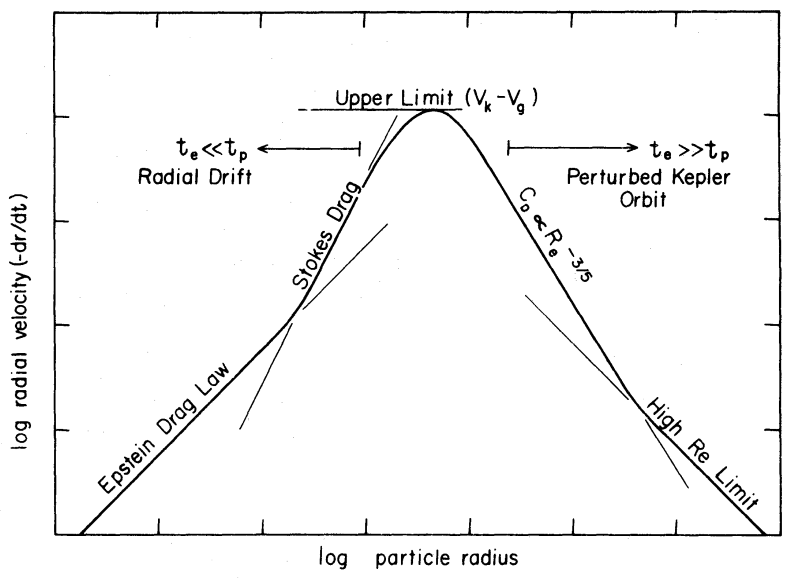
\includegraphics[width=0.9\textwidth]{figures/chap1_drift.png}
   \caption{Schematyczny rysunek zależności pomiędzy rozmiarem ziaren pyłu, a
   maksymalną prędkością radialnego dryfu. Obrazek pochodzi z
   pracy~\cite{W77}}
   \label{fig:chap1_drift}
\end{figure}

Ziarna te są w stanie osiągać prędkości radialne rzędu
$10^2\div10^3\cm\s^{-1}$~\cite{W77}, co przekłada się na utratę
tych cząstek w skali czasowej rzędu setek lat!  Kolejną konsekwencją zależności
radialnego dryfu od rozmiaru cząstek jest zróżnicowanie ich prędkości względem
siebie. Cząstki pyłu sklejają się dzięki oddziaływaniom międzycząsteczkowym,
które są szczególnie wydajne w przypadku małych cząstek i dużego ich
zagęszczenia. Wraz ze wzrostem cząstek proces zlepiania zachodzi coraz wolniej.
Koagulacja faworyzuje małe cząstki, które mają większy stosunek powierzchni do
masy. Przy odpowiednio niskiej prędkości względnej kolizje prowadzą do tworzenia
coraz to większych aglomeratów cząstek~\citep{BW08}, ale dla dużych różnic w
prędkościach najbardziej prawdopodobnym rezultatem zderzenia jest
fragmentacja bądź odbicie~\citep{Z10}. 
\par Nie dość, że czas dla którego możemy oczekiwać dynamicznej ewolucji pyłu o
rozmiarach $0.1 \div 10\m$ jest niezmiernie krótki, to nie jesteśmy w stanie
wskazać żadnego mechanizmu powodującego dalszy wzrost rozmiarów pyłu. Problem
ten nosi nazwę \emph{metrowej bariery wzrostu} i jest najważniejszą
niewyjaśnioną kwestię obecnego paradygmatu formacji planet.
\par W ogólności dryf radialny przemieszcza pył w kierunku maksimum ciśnienia w
gazie. Dla modelu spokojnego dysku jest to tożsame z centrum grawitacji. Należy
jednak pamiętać, że turbulentny ośrodek może wytwarzać lokalne, przejściowe
maksima w ciśnieniu gazu, dla których gradient będzie dużo większy niż gradient
globalny. Z tego względu obszary o podwyższonym ciśnieniu będą działać jako
swoiste pułapki na pył, przejściowo zwiększając jego gęstość. 
Cuzzi, Hogan \& Shariff~\citep{CHS08} postulują, iż przejściowe zagęszczenia
pyłu na skutek ruchów turbulentnych są wyzwalaczem dla dalszych procesów
formowania się planetezymali.
\begin{figure}
   \centering
   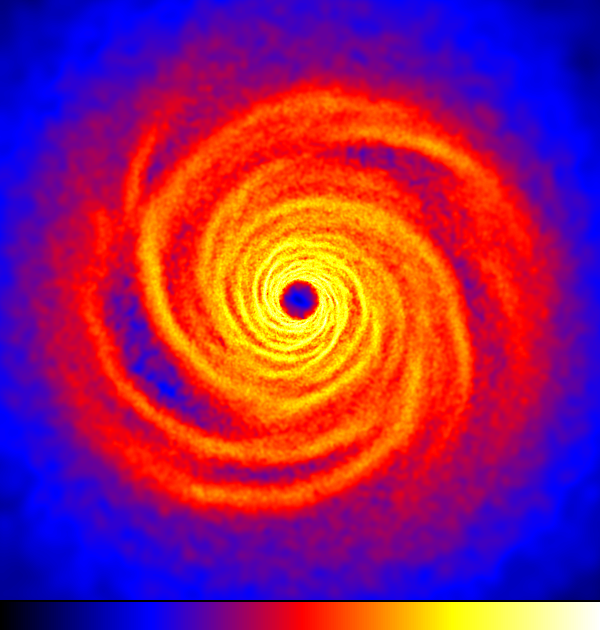
\includegraphics[width=0.49\textwidth]{figures/chap1_gasdisk.png}
   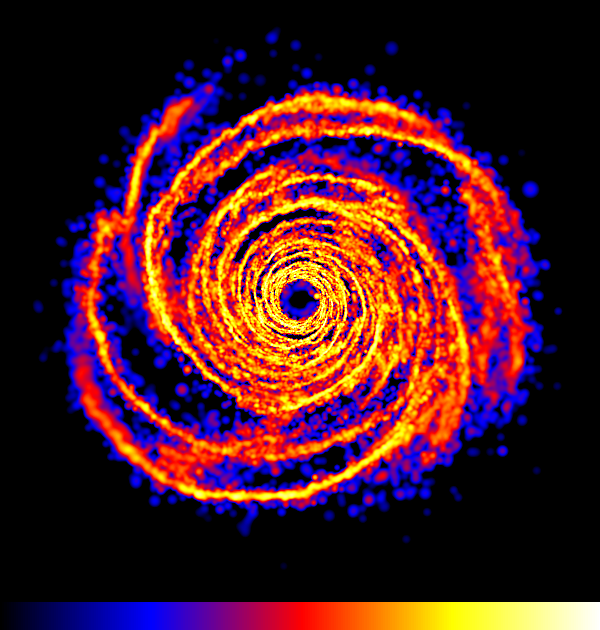
\includegraphics[width=0.49\textwidth]{figures/chap1_dustdisk.png}
   \caption{Symulacja dwuskładnikowego, izotermicznego dysku protoplanetarnego,
      lewy panel przedstawia rozkład ciśnienia gazu, prawy zaś rozkład gęstości
      gazu.  Wyraźnie widać jak pył jest pułapkowany w lokalnych maksimach
      ciśnienia. Obrazek pochodzi z pracy~\cite{RLP2006}}
   \label{fig:chap1_trap}
\end{figure}

\subsection{Sedymentacja i niestabilność Kelvina-Helmholtza (KHI)}
W dotychczasowych rozważaniach pominęliśmy wpływ pionowej składowej siły
grawitacji pochodzącej od gwiazdy macierzystej na dynamikę ziaren pyłu. O ile
gaz zostaje ściśnięty przez grawitację do momentu osiągnięcia równowagi z
gradientem ciśnienia~\mref{eq:zeq}, o tyle opadaniu pyłu nie przeciwdziała żaden
proces fizyczny~\footnote{na chwilę pomińmy fakt, że gaz jest ośrodkiem
turbulentnym i przez wzajemne sprzężenie wpływa na dynamikę pyłu}. Sedymentacja
mogłaby zatem prowadzić do wytworzenia się cienkiej i bardzo gęstej warstwy
pyłu, która po przekroczeniu wartości krytycznej rozpadłaby się pod własnym
ciężarem~\citep{GW73}. Zauważmy jednak, że
osiadanie pyłu prowadzi do stopniowego zwiększenia stosunku pyłu do gazu w
płaszczyźnie dysku. Ponadto jak już było wspomniane pył porusza się na wybranej
orbicie z prędkością keplerowską, natomiast gaz pod wpływem radialnego gradientu
ciśnienia z prędkością pod keplerowską. Duża koncentracja pyłu w płaszczyźnie
powoduje, że gaz jest efektywniej ,,pchany'' przez pył i zaczyna poruszać się
szybciej niż warstwy gazu leżące poniżej i powyżej płaszczyzny rotacji dysku.
Prowadzi to do pionowego gradientu prędkości azymutalnej gazu, co stanowi
konfigurację niestabilną ze względu na niestabilność Kelvina-Helmholtza i
prowadzi do wzbudzenia się turbulencji w gazie. Na skutek wzajemnego sprzężenia
turbulencja propaguję się na składnik pyłowy i hamuje sedymentację~\cite{JHK06}.
Ostatnie badania pokazują że tylko odpowiednio masywne i metaliczne dyski są nie
wrażliwe na ten proces~\citep{L10}. Podobnie jak w przypadku niestabilności
magnetorotacyjnej turbulentne ruchy gazu skutkują analogicznymi ruchami pyłu,
jednakże i w tym wypadku ustala się pewien stan równowagi między sedymentacją
pyłu, a turbulencją. 

\subsection{Niestabilność strumieniowa}
Działania niestabilności dla gazu w dysku protoplanetarnym może sformować
się warstwa pyłu o skończonej grubości, dużo mniejszej niż grubość dysku
gazowego. Pył ten jest jednak zbyt rzadki, aby wzbudziła się w nim
niestabilność grawitacyjna.
\par Pomimo tych niesprzyjających warunków istnieje proces który dominuje
ewolucję pyłu w momencie w którym stosunek koncentracji ziaren pyłu do gęstości
gazu zbliża się do jedności. Tym mechanizmem jest {\it niestabilność
strumieniowa} po raz pierwszy przedstawiona w pracy~\cite{YG05}.  Wraz ze
wzrostem gęstości pyłu spowodowanego jego dryfem w kierunku najbliższego
maksimum ciśnienia gazu, wzrasta wypadkowa siła z jaką pył oddziałuje na gaz.
Prowadzi to zwiększenia prędkości gazu i wzrostu ciśnienia na skutek zagarniania
obszarów gazów poruszających się wolniej. Zwiększa to maksimum ciśnienia w gazie
i przyspiesza dryft pyłu z otaczających go obszarów. Normalnie gradient ciśnienia
skierowany na zewnątrz gęstniejącego obszaru powodowałby jego szybkie rozmycie,
ale w wypadku rotującego dysku połączenie ciągłego dryfu pyłu i siły Coriolisa
prowadzi do wytworzenia się równowagi geostroficznej~\cite{JBL11}. Nasycenie
gęstości pyłu następuje w momencie gdy masa porcji pyłu jest w stanie wyrwać się
z lokalnego maksimum gazu.  Nawet zaniedbując efekt samograwitacji w trakcie
ewolucji niestabilności strumieniowej lokalna gęstość pyłu może zwiększyć się
tysiąckrotnie~\cite{JY07}, co może prowadzić do wytworzenia się grawitacyjnie
związanych obiektów~\cite{J07}. Ostatnie badania niestabilności strumieniowej
skupiały się na różnych aspektach fizycznych które mają wpływ na jej rozwój
t.j.: uwzględnienie szerokiego spektrum rozmiaru cząstek pyłu~\cite{BS10a},
wpływ globalnego gradientu ciśnienia w dysku okołogwiazdowym~\cite{BS10b},
stratyfikacja dysku~\cite{T12}. Niemniej jednak wszystkie publikacje naukowe
były ograniczone do lokalnego przybliżenia dysku.

\section{Cel pracy}
Głównym celem pracy jest zbadanie niestabilności strumieniowej w bardziej
realistycznym przybliżeniu radialnie rozciągłego dysku.

Celem badań jest oszacowanie i opis wpływu niestabilności strumieniowej na
proces generowania lokalnego wzrostu stosunku gęstości pyłu do gazu w globalnym
dysku pyłowo-gazowym. Pył jako ważny składnik dysku okołogwiazdowego można
opisywać w przybliżeniu płynowym (funkcja już zaimplementowana w kodzie PIERNIK
patrz (Hanasz, et al. 2009b) lub w przybliżeniu punktów materialnych. Obecnie w
literaturze naukowej dominuje druga  metoda, ważne jest więc sprawdzenie
jakościowych i ilościowych różnic obu podejść w globalnych symulacjach
niestabilności strumieniowej. 



%%%%%%%%%%%%%%%%%%%%%%%%%%%%%%%%%%%%%%%%%%%%%%%%%%%%%%%%%%%%%%%%%%%%%%%%%%%%%%%%
% vim: tw=80 ts=3: 
